\section{RESULTADOS}


\subsection{Invasibilidad}
Dada la parametrizaci\'on usada y asumiendo :
\begin{enumerate}
\item $\beta_R = \beta_C = \beta_P = \beta$
\end{enumerate}

Derivamos expl\'icitamente las siguientes condiciones para cada criterio de invasibilidad \textbf{I} y zona \textbf{Z(I)} asociada a \textbf{I} en funci\'on a $k_{\RC},k_{\CP}$ y $m_P$.

\subsubsection{C $\to$ R}

\begin{equation}
  \frac{dC}{dt} >0 \iff  m_P^{h_R +1 - 2\beta} > \zeta_1(k_{\RC},k_{\CP}) = k_{\CP}^{2\beta -1 -h_R}(\frac{\chi_1}{\chi_0})
\end{equation}
Donde:
\begin{equation}
  \begin{aligned}
    h_R &= p_v + 2(D_R - 1)p_d \\
    \chi_0 &= \varepsilon_1 \kappa_0\alpha_{0,1} g(k_{\RC}) \\
    g(k_\RC) &= f_1(k_{\RC})k_{\RC}^{1-\beta}\\
    \chi_1 &= q_{0,1} 
  \end{aligned}
\end{equation}
Entonces:
\begin{equation}
\mathbf{Z(I_{\C\to \R})} := \{ (k_{\RC},k_{\CP},m_P) \in \mathbb{R}^3_+ / m_p^{h_R + 1 - 2\beta} > \zeta_1(k_{\RC},k_{\CP}) \}
\end{equation}


Dada la relaci\'on anterior, podemos deducir la influencia de los par\'ametros del modelo sobre la invasibilidad de $C$.\\

En particular dado que $f_1(k_{\RC}) \to 0 (k_{\RC} \to 0)$ y $\beta <1$ tenemos que $\chi_0 \to 0 (k_{\RC} \to 0)$,para un valor acotado de $\kappa_0$,y por lo tanto valores extremadamente peque\~nos de $k_{\RC}$ siempre ser\'an exclu\'idos de $\mathbf{Z(I_{\C\to \R})}$ si mantenemos $m_P$ y $k_{\CP}$ constante(un comportamiento an\'alogo se observa para $k_\CP$ peque\~nos), dicho esto al aumentar $k_{\CP}$, $\kappa_0$ y $m_P$ el m\'inimo $k_{\RC}$ disminuye, asu ves dado que el impacto de $m_P y k_\CP$ esta influenciado por la dimensi\'on del espacio de b\'usqueda esta disminuci\'on es mas fuerte para ambientes $3D$.\\

Para valores fijos de $k_{\CP}, \kappa_0 ,m_P$,el valor m\'aximo de $k_{\RC}$ en $\mathbf{Z(I_{\C\to \R})}$ depender\'a del valor de $\phi$ y $fm$. Sin embargo para los distintos $fm$ tenemos un comportamiento cualitativo similar , debido a la similitud existente entre $f_1$ para distintos $fm$(v\'ease anexos). Dado la similitud entre $g$ y $f_1$ por un tratamiento similar al descrito en anexos podemos observar que para $\phi$ \emph{suficientemente peque\~no} $\chi_0$ crece mon\'otonamente con respecto a $k_\RC$ por lo tanto se observa la presencia de un valor umbral $k$ tal que por encima de \'el la invasi\'on de $C$ es posible. A su vez para valores de $\phi$ \emph{suficientemente grandes} tenemos que $\chi_0$ presenta un valor m\'aximo por encima del cual decrece mon\'otonamente, es m\'as $\chi_0 \approx c k_{RC}^{h - \phi}$ para valores de $k_\RC$ elevados(donde $h$ depende de $fm$) y por tanto estos ser\'ian exclu\'idos de $\mathbf{Z(I_{\C\to \R})}$ dado que al mantener $m_P$ y $k_\CP$ fijos cambios en $k_\RC$ simplemente indican cambios en la masa de $m_R$ podemos interpretar estos resultados de la siguiente manera, sin importar $\phi$, $m_R$ tiene que tener un tama\~no m\'inimo el cual permita a $C$ invadir, esto debido al hecho que $m_R$ influencia la capacidad de carga de $R$, y por ende la energ\'ia disponible a $C$ al momento de la invasi\'on, sin embargo valores elevados de $m_R$ son inviables para $C$ para $\phi$ \emph{suficientemente grandes} ya que en estos casos a pesar de que el sistema presenta una gran cantidad de energ\'ia disponible, debido a la baja probabilidad de captura de $R$ por parte de $C$ no se traducen en aumentos en biomasa de $C$, es decir lo importante para $C$ al momento de la invasi\'on no solamente es la energ\'ia total presente en el sistema sino que \'esta se encuentre en una \emph{forma} que pueda ser explotada por $C$.\\


Si mantenemos $\kappa_0,k_\CP$ y $k_\RP$ fijos, observamos que para que sea posible la invasi\'on de $C$, $m_P$ tiene que superar un valor dado. Dado que aumentos en $m_P$ para size ratios fijos implican aumentos en las masas de $R$ y $C$ respectivamente, esto nos dice que existe un tama\~no de $C$ y$R$ por encima del cual la invasi\'on de $C$ es posible.

La dimensi\'on del espacio de b\'usqueda afecta positivamente a $\chi_0$(si asociamos cambios en $\kappa_0$, y con $k_\RC > 10^{-30}$), sin embargo debido a que aumenta $h$ su impacto total sobre la invasibilidad puede ser negativo para valores elevados de $k_\RC$(i.e cuando el m\'inimo $k_\RC$ necesario para la invasi\'on es elevado, como se da para $k_\CP$ y $m_P$ peque\~nos), siendo m\'as precisos siempre que $\frac{\chi_1}{\chi_0} >1$ en ambientes $2D$ tenemos que el impacto es positivo, pero para $\frac{\chi_1}{\chi_0} < 1$ el impacto es negativo si $ (\frac{\chi_1}{\chi_0})_{3D}^\frac{1 + h_{2D} - 2 \beta}{1 + h_{3D} - 2 \beta} >  (\frac{\chi_1}{\chi_0})_{2D} $.\\


\begin{figure}
  \centering
  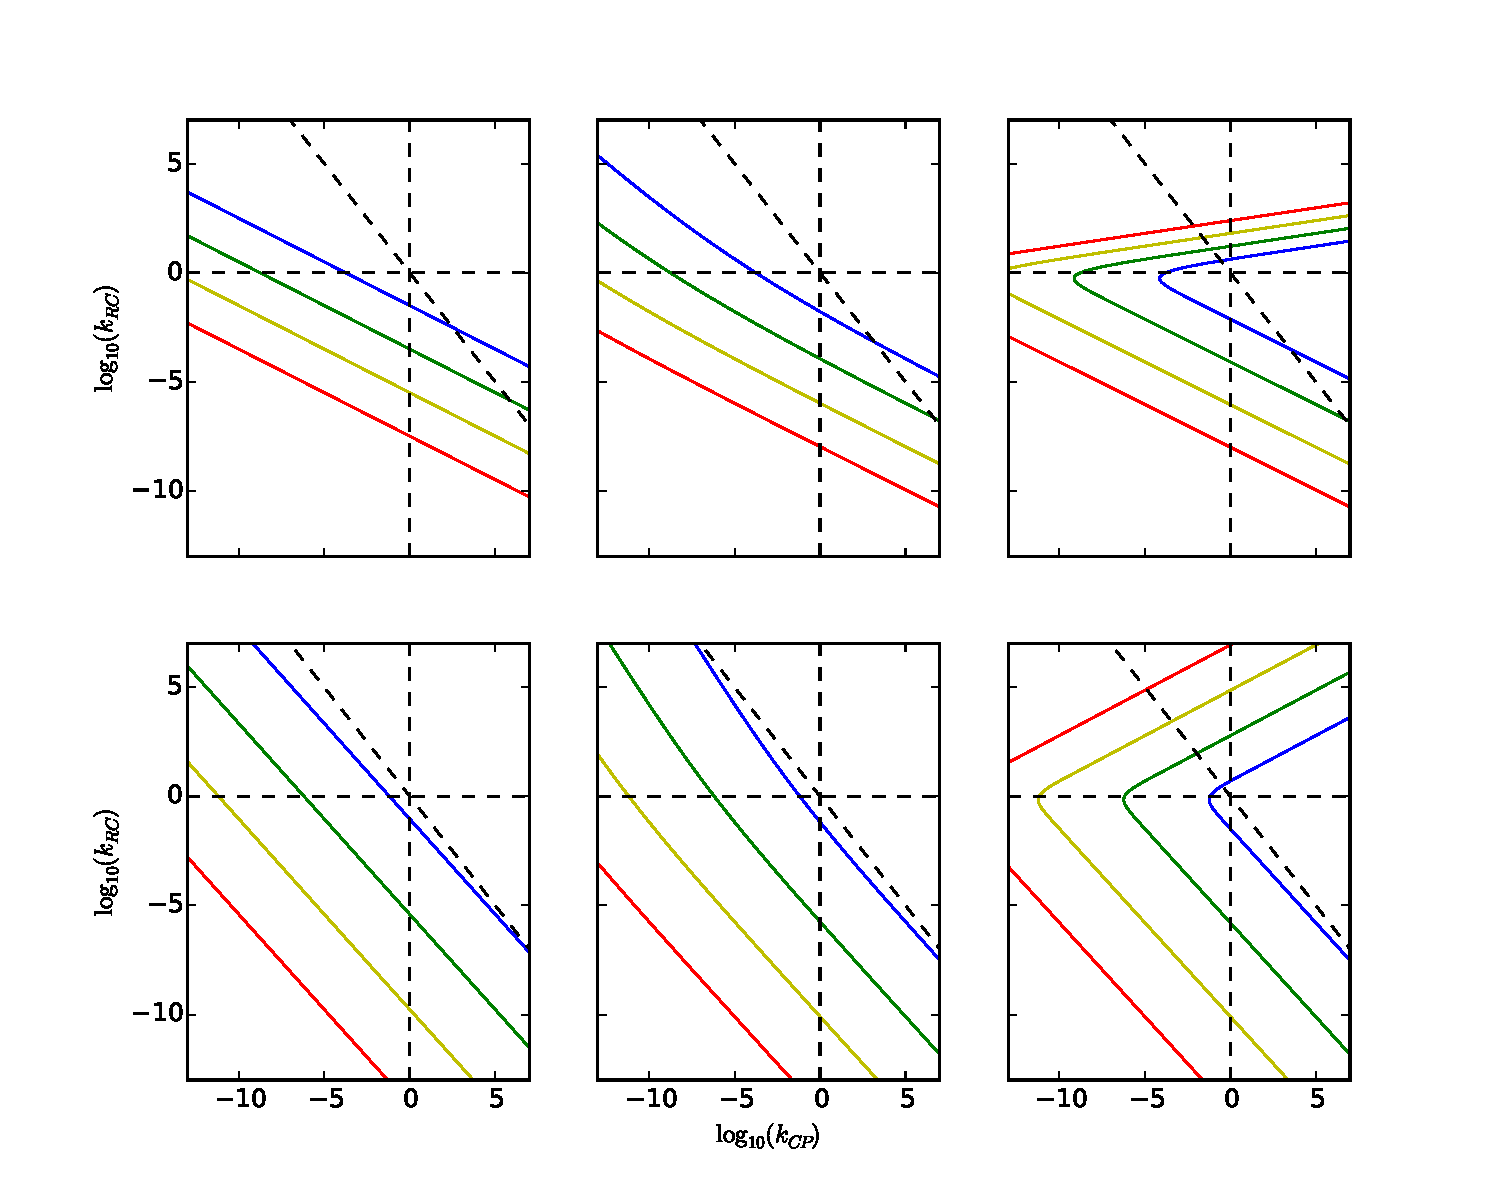
\includegraphics[width = 0.99\textwidth]{./Plots/Z(IC2)AcGrGr.pdf}
  \caption[Env $Z(IC2)$]{\emph{Envolturas de Invasibilidad} para el caso de el depredador intermedio $C$ como invasor frente a una comunidad receptora formada por $R$. La fila superior es para espacios de b\'usqueda bidimensionales y la inferior tridimensionales, las columnas de izquierda a derecha aumentan el valor de $\phi$, siendo $0.02,0.2$ y $2$ respectivamente.Las diferentes lineas implican distintas masas de depredador $m_P$ :({\hwplotR}) $10^5 kg$,  ({\hwplotY}) $1kg$, ({\hwplotG}) $10^{-5}kg$ y ({\hwplotB}) para $10^{-10}kg$. ({\hwplotK}) separa las zonas donde $K_{RC},K_{CP},k_{RP}$ son mayores o menores que 1 respectivamente. $k_0 = 0.1$ y $k_0 = 30$ para el caso $2D$ y $3D$ respectivamente, los valores de los otros par\'ametros son los descritos en el anexo \ref{subsec:params}}
  \label{fig:Z(IC2)}
\end{figure}

\subsubsection{P $\to$ R}

\begin{equation}
  \frac{dP}{dt} >0 \iff  m_P > \zeta_2(k_{\RC},k_{\CP}) = (\frac{q_{0,2}}{\eta_0})^{\frac{1}{h_R +1 - 2\beta}}
\end{equation}
Donde:
\begin{equation}
  \begin{aligned}
    \eta_0 &= \varepsilon_2 \kappa_0\alpha_{0,2} f_2(k_{\RP})k_{\RP}^{1-\beta} \\
  \end{aligned}
\end{equation}

\begin{equation}
\mathbf{Z(I_{\PP \to \R})} := \{ (k_{\RC},k_{\CP},m_P) \in \mathbb{R}^3_+ / m_p > \zeta_2(k_{\RC},k_{\CP}) \}
\end{equation}

El comportamiento es similar al descrito anteriormente, reemplazando $k_\RC$ por $k_\RP$ en nuestra discusi\'on anterior.


\begin{figure}
  \centering
  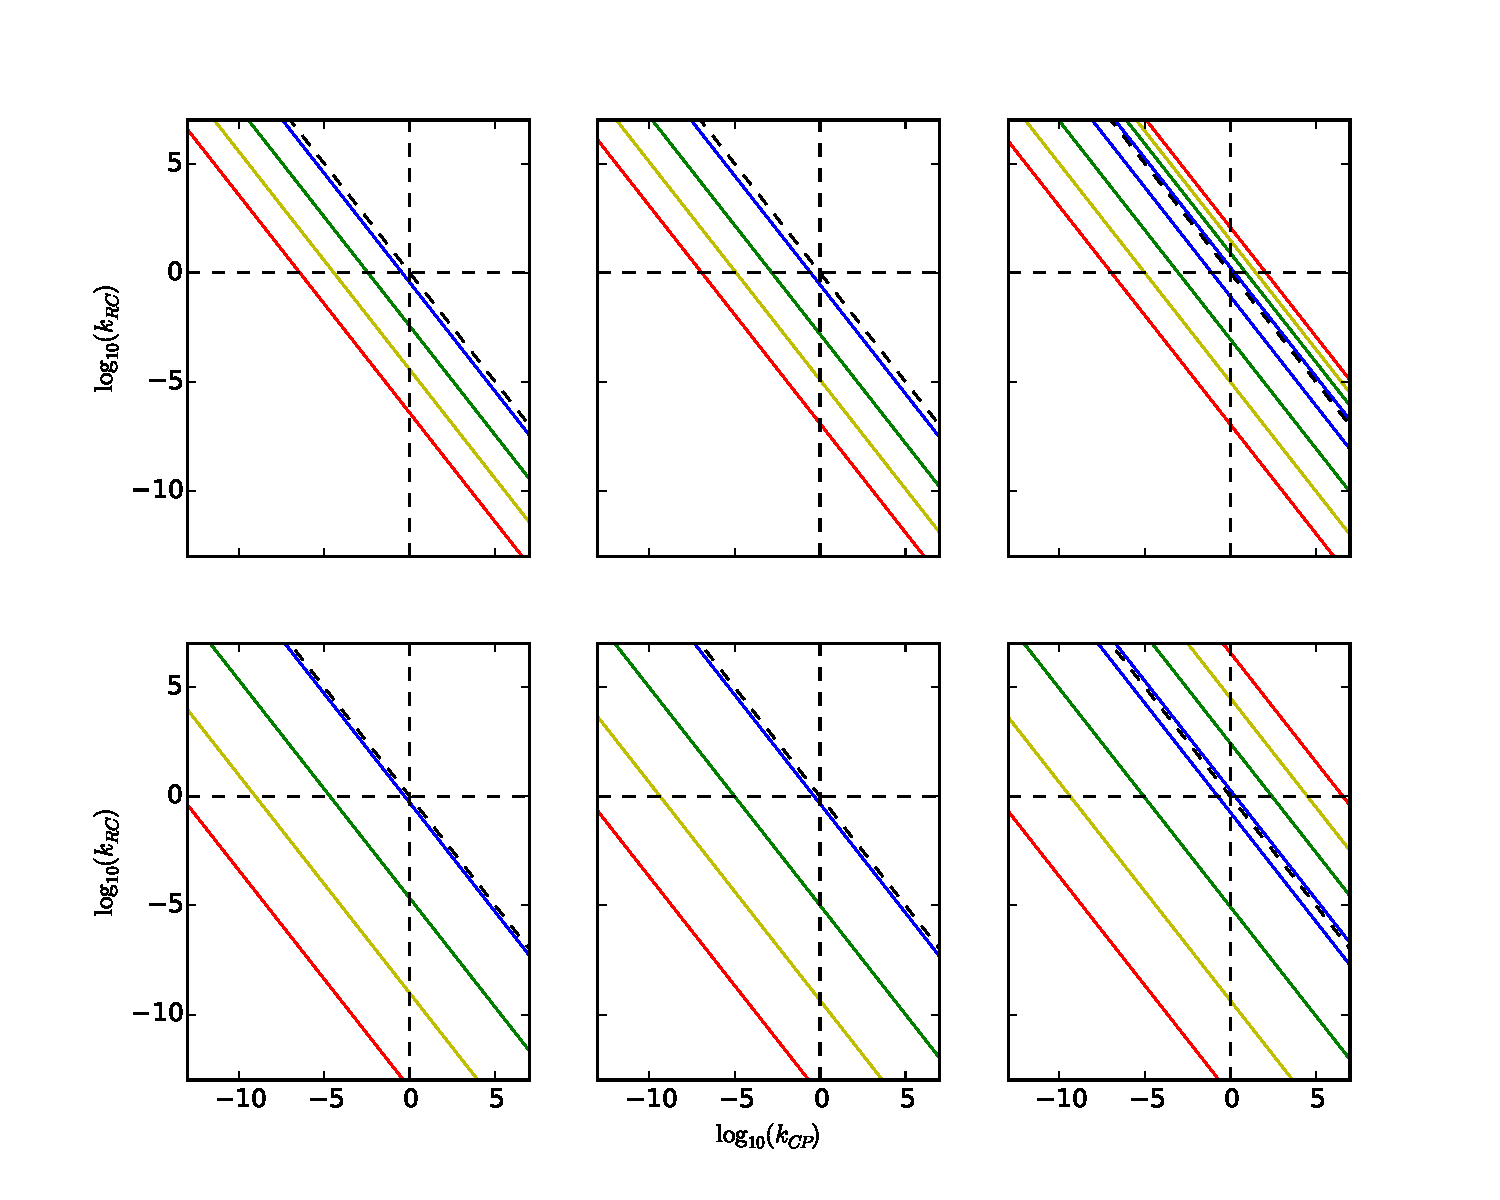
\includegraphics[width = 0.99\textwidth]{./Plots/Z(IC3)AcGrGr.pdf}
  \caption[Env $Z(IC2)$]{\emph{Envolturas de Invasibilidad} para el caso de el depredador intermedio $P$ como invasor frente a una comunidad receptora formada por $R$.Las dem\'as especificaciones se comparten con la figura ~\ref{fig:Z(IC2)}}
  \label{fig:Z(IC3)}
\end{figure}


Asumiendo a su vez que $D_R = D_C = D$

Definamos:
\begin{equation}
  h = p_v + 2(D-1)p_d
\end{equation}

\subsubsection{P $\to$ C-R}
\begin{equation}
  \frac{dP}{dt}  >0 \iff \xi_3 + \xi_4 - q_{0,2} >0 \land m_P > \zeta_3(k_{\RC},k_{\CP}) = (\frac{\xi_4\xi_2}{\xi_3 + \xi_4 - q_{0,2}})^{\frac{1}{h + 1 - 2\beta}}
\end{equation}

Donde:
\begin{equation}
  \begin{aligned}
    \xi_0 &= \frac{q_{0,1} k_{\CP}^{\beta - h}}{\epsilon_1 \alpha_{0,1} f_1(k_{\RC})}\\
    \xi_1 &= \frac{r_0 k_{\CP}^{\beta-h}}{\alpha_{0,1} f_1(k_{\RC})k_{\RC}^{1-\beta}}\\
    \xi_2 &= \frac{\xi_0}{k_0 k_{\RP}^{1-\beta}} \\
    \xi_3 &= \varepsilon_2 \alpha_{0,2} f_2(k_{\RP}) \xi_0\\
    \xi_4 &=\varepsilon_3 \alpha_{0,3} f_3(k_{\CP}) \xi_1
  \end{aligned}
\end{equation}

Por lo tanto 
\begin{equation}
\mathbf{Z(I_{\PP \to \C-\R})} := \{ (k_{\RC},k_{\CP},m_P) \in \mathbb{R}^3_+ / m_p > \max\{\zeta_1(k_{\RC},k_{\CP}),\zeta_3(k_{\RC},k_{\CP})\} \}
\end{equation}

A diferencia de los dos casos anteriores la complejidad de esta expresi\'on imposibilita un an\'alisis a la misma profundidad que el descrito anteriormente, y simplemente nos referimos a ciertos casos particulares.\\

La primera de las condiciones es:
\begin{equation}
  \xi_3 + \xi_4 > q_{0,2}
\end{equation}

Dado que $\xi_3$ esta relacionado con la tasa de consumci\'on del recurso basal y $\xi_4$ con la tasa m\'axima de consumci\'on sobre el consumidor intermedio(i.e la tasa de consumci\'on a la m\'axima abundancia para $C$) esta relaci\'on concuerda con la intuici\'on de la existencia de un nivel de energ\'ia m\'inimo para la invasi\'on de $P$, y donde $\xi_3 + \xi_4$ esta relacionado con la maxima energ\'ia disponible para el invasor $P$.
En general tenemos :
\begin{equation}
  \begin{aligned}
    \xi_3 = a_0 \frac{f_2(k_\RP)}{f_1(k_\RC)} k_\CP^{\beta-h} \\
    \xi_4 = a_1 \frac{f_3(k_\CP)}{f_1(k_\RC)} \frac{k_\CP^{\beta - h}}{k_\RC^{1-\beta}}
  \end{aligned}
\end{equation}

Donde :
\begin{equation}
  \begin{aligned}
    a_0 = \frac{\varepsilon_2 \alpha_{0,2} q_{0,1}}{\varepsilon_1 \alpha_{0,1}} \\
    a_1 = \frac{\varepsilon_3 \alpha_{0,3} r_0}{\alpha_{0,1}}
  \end{aligned}
\end{equation}

Definiendo $g_1:= f_1 k_\RC^{1-\beta} g_2:= f_2 k_\CP^{\beta- h} , g_3 := f_3 k_\CP^{\beta-h} $ , para $\phi$ \emph{suficientemente peque\~no} tenemos que las tres funciones son mon\'otonas y para $\phi$ \emph{suficientemente grande} tenemos que son \emph{unimodales}.\\

En el siguiente argumento siempre que nos referimos al comportamiento respecto a un $size-ratio$ mantenemos el otro fijo.\\

\begin{tabular}{p{1.5in}|m{1.5in}|m{1.5in}} 
 & Mon\'otonas  & Unimodales \\
$\lim_{k_\CP \to \infty} \xi_3$ & $+\infty$  & 0 \\
$\lim_{k_\CP \to \infty} \xi_4$ & $+\infty$  & 0 \\
$\lim_{k_\RC \to \infty} \xi_4$ & 0  & $+\infty$ \\
$\lim_{k_\CP \to 0} \xi_3$ & 0 & 0 \\
$\lim_{k_\CP \to 0} \xi_4$ & 0 & 0 \\
$\lim_{k_\RC \to 0} \xi_4$ & $+\infty$ & $+\infty$ \\
\end{tabular}

En el caso que las funciones sean mon\'otonas tenemos que la condici\'on se cumple para $k_\CP$ suficientemente grande y $k_\RC$ suficientemente peque\~no, y no se cumple para $k_\CP$ suficientemente peque\~nos. En el segundo caso la condici\'on no se cumple si $k_\CP$ es demasiado grande o peque\~no y se cumple si $k_\RC$ es suficientemente peque\~no o grande.\\

A su vez tenemos:
\begin{equation}
  \lim_{k_\RC \to \infty} \xi_3 = a_0 k_\CP^{\beta - h - \phi} \lim_{k_\RC \to \infty} \frac{h_2(k_\RP)}{h_1(k_\RP)} 
\end{equation}

Donde $h_i = \frac{f_i}{\Pi_i}$ y en el caso espec\'ifico de la combinaci\'on de estrategias $Gr-Gr-Ac$ tenemos: $\lim_{k_\RC \to +\infty} \xi_3 = a_0 k_\CP^{\beta -h + (D-1)p_d - \phi}$ luego para funciones mon\'otonas la condici\'on se cumple para $k_\RC$ \emph{suficientemente grande} y $k_\CP$ fijo siempre que $k_\CP^{\beta - h + (D-1)p_d - \phi} > \frac{q_{2,0}}{a_0}$, esta \'ultima condici\'on esta influenciada por la dimensi\'on del espacio de b\'usqueda ya que $ \beta - h + (D-1)p_d - \phi >0$ para espacios $2D$ y menor para espacios $3D$. Las otras dos combinaciones de estrategias se comportan de forma similar.\\

Para valores intermedios la situaci\'on es m\'as dif\'icil de describir y nos referimos a la figura  ~\ref{fig:NC_PCR}, donde se observa que el comportamiento asint\'otico en cierta manera se manifiesta a este nivel, teniendo para valores peque\~nos de $\phi$ y $k_\RC$ fijo un valor de $k_\CP$ a partir del cual la condici\'on se cumple, y caso contrario a valores altos de $\phi$, a su vez para $k_\CP$ fijo tenemos un valor de $k_\RC$ debajo del cual la condici\'on se cumple.Para $\phi$ elevado y $k_\RC$ elevado tenemos que la condici\'on se cumple a\'un para $k_\CP$ peque\~nos. A su vez se observan las diferencias existentes entre espacios de b\'usqueda de diferente dimensi\'on y distintas estrategias de forrajeo las cuales como se mencion\'o previamente comparten en gran medida el comportamiento cualitativo respecto a cambios en la raz\'on de masas.

\begin{figure}
  \centering
  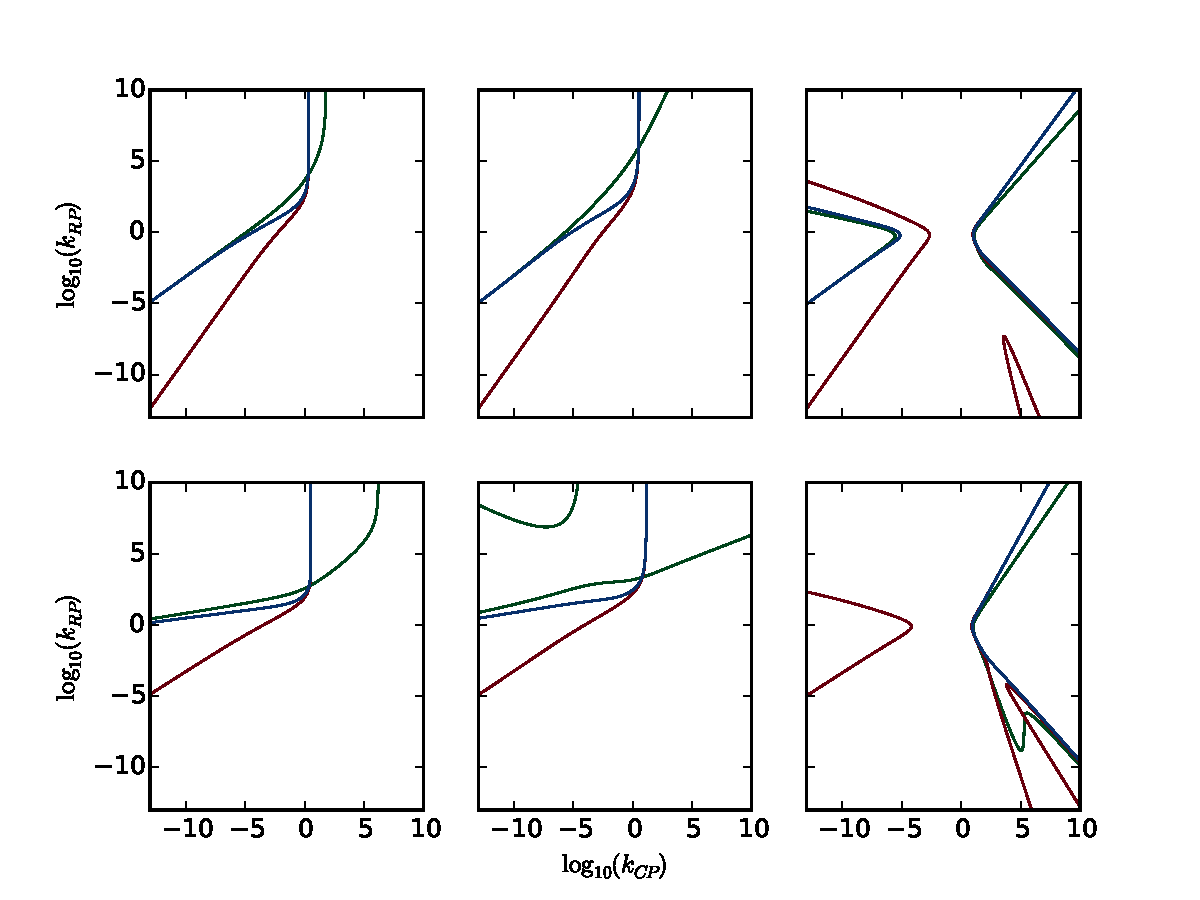
\includegraphics[width = 0.99\textwidth]{./Plots/NecessityPCR.pdf}
  \caption[Condiciones Necesarias $P \to C-R$]{Condiciones necesarias para la invasibilidad del depredador tope $P$ sobre el subsistema $C-R$.Para las estrategias de forrajeo:({\hwplotR}) $Ac-Sw-Sw$, ({\hwplotG}) $Gr-Gr-Ac$ y ({\hwplotB}) $Ac-Ac-Ac$. La fila superior se refiere a ambientes $2D$ y la inferior a $3D$, de izquierda a derecha tenemos $\phi : 0.02,0.2 y 2$. $k_0= 0.1,30$ en ambientes $2D$ y $3D$ respectivamente.}
  \label{fig:NC_PCR}
\end{figure}

En el caso de la segunda condici\'on asumimos que los valores de $k_\RC , k_\CP , m_P$ son tales que es posible la invasi\'on de $C$(es decir todas las restricciones descritas para la invasibilidad de $C$ ya se aplican, en particular $\kappa_0$ afecta positivamente el cumplimiento de esta condici\'on), reescribiendo la condici\'on anterior observamos que $\xi_2$ es justamente $\zeta_1(k_{\RC},k_{\CP})$ y por ende tenemos que $m_P^{1 + h - 2\beta} > \xi_2$ , y en este caso tendr\'iamos que la condic\'on se seguir\'ia cumpliendo siempre que $\frac{\xi_4}{\xi_3 + \xi_4 - q_{0,2}} \leq 1$ y una condici\'on suficiente para que se cumpla es $ \xi_3 \geq q_{0,2}$, lo que se traduce biol\'ogicamente a que todas las necesidades energ\'eticas del invasor son cubiertas por el recurso $R$.\\

Usando la tabla desarrollada anteriormente vemos que dependiendo de la forma de las funciones, se seleccionan distintos valores de $k_\CP$ y $k_\RC$. Para funciones mon\'otonas para $k_\RC$ fijo existe un $k_\CP$ a partir del cual la condici\'on se cumple , y en el caso de funciones unimodales la condici\'on no se cumple para $k_\CP$ \emph{suficientemente grande o peque\~no}. Tomando igual que en el caso anterior la combinaci\'on de estrategias de forrajeo $Gr-Gr-Ac$ tenemos que 
\begin{equation}
  \lim_{k_\RC \to 0} \xi_3 = a_0 k_\CP^{\beta - h + (D-1)p_d}  \ \ \land \lim_{k_\RC \to 0 \infty} \xi_3 = a_0 k_\CP^{\beta -h + (D-1)p_d - \phi} 
\end{equation}
Denotando $u_1 = \beta - h + (D-1)p_d$ tenemos que $ u_1 >0$ para espacios de b\'usqueda $2D$ y menor que cero en espacios $3D$ por tanto tenemos que la condici\'on se cumple para $k_\RC$ peque\~nos , en espacios $2D$ siempre que $k_\CP$ es suficientemente grande y lo contrario ocurre en ambientes $3D$ donde se requiere que $k_\CP$ sea peque\~no. De forma similar podemos analizar el comportamiento para un $k_\CP$ fijo cuando $k_\RC$ es elevado , para $\phi$ peque\~nos tenemos que la condici\'on es an\'aloga a la anterior, se cumple en $2D$ para $k_\CP$ elevados y en $3D$ a $k_\CP$ bajos ; para $\phi$ grande tenemos que la condici\'on se cumple siempre que $k_\CP$ es suficientemente peque\~no.\\
En caso que esta condici\'on no se cumpla , la masa $m_P$ necesaria para cumplir la condici\'on ser\'a mayor que en el caso de la invasi\'on de $C$ a $R$.\\

Este criterio comparte una propiedad cualitativa con los dos anteriores, siempre que el par de size ratios cumplan con la primera condici\'on exisitira un valor de $m_P$ por encima del cual la invasi\'on es posible. Curvas de nivel para distintos valores de $m_P$ se representan en la figura ~\ref{fig:Z(IC4)}, donde se aprecia que el espacio de combinaciones posibles de size ratios para los cuales la invasi\'on es posible aumenta con respecto a $m_P$(un comportamiento similar se observa respecto a $\kappa_0$).


\begin{figure}
  \centering
  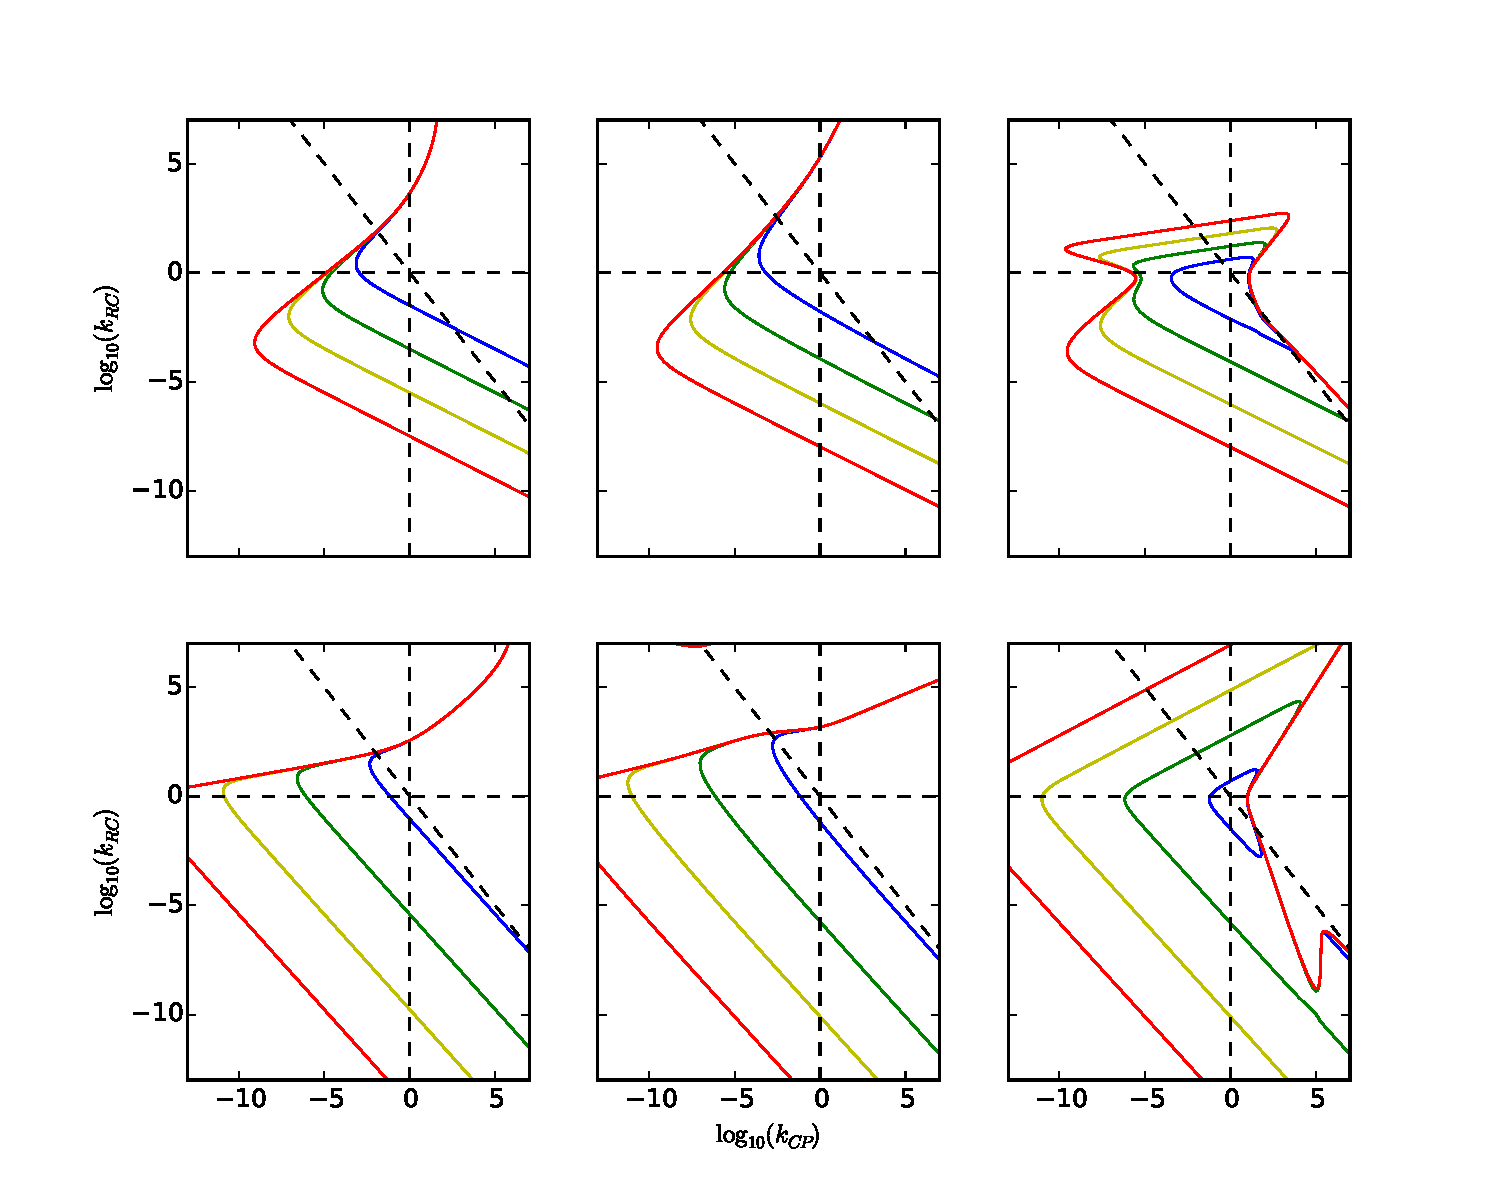
\includegraphics[width = 0.99\textwidth]{./Plots/Z(IC4)AcGrGr.pdf}
  \caption[Env $Z(IC4)$]{\emph{Envolturas de Invasibilidad} para el caso de el depredador tope $P$ como invasor frente a una comunidad receptora formada por $R-C$ .Las dem\'as especificaciones se comparten con la figura ~\ref{fig:Z(IC2)}}
  \label{fig:Z(IC4)}
\end{figure}


\subsubsection{C $\to$ P-R}
\begin{equation}
  \frac{dC}{dt}  >0 \iff \gamma_5 + \gamma_4 - \gamma_3 < 0 \lor  m_P < \zeta_4(k_{\RC},k_{\CP}) = (\frac{\gamma_4\gamma_2}{\gamma_5 + \gamma_4 - \gamma_3})^{\frac{1}{h + 1 - 2\beta}}
\end{equation}

Donde:
\begin{equation}
  \begin{aligned}
    \gamma_0 &= \frac{q_{0,2}}{\varepsilon_2 \alpha_{0,2} f_2(k_{\RP})}\\
    \gamma_1 &= \frac{r_0 k_{\RP}^{\beta -1}}{\alpha_{0,2} f_2(k_{\RP})}\\
    \gamma_2 &= \frac{\gamma_0}{\kappa_0 k_{\RP}^{1-\beta}} \\
    \gamma_3 &= \varepsilon_1\alpha_{0,1} f_1(k_{\RC}) k_{\CP}^{h -1} \gamma_0\\
    \gamma_4 &=\alpha_{0,3} f_3(k_{\CP}) \gamma_1 \\
    \gamma_5 &= q_{0,1} k_{\CP}^{\beta-1}
  \end{aligned}
\end{equation}

Por lo tanto:

\begin{equation}
\mathbf{Z(I_{\C \to \PP-\R})} := \{ (k_{\RC},k_{\CP},m_P) \in \mathbb{R}^3_+ / \zeta_4(k_{\RC},k_{\CP}) > m_p > \zeta_2(k_{\RC},k_{\CP}) \}
\end{equation}

Reescribiendo la primera de las condiciones:
\begin{equation}
  \gamma_3 - \gamma_4 - \gamma_5 >0 \iff \xi_3 + c \xi_4 < q_{2,0}
\end{equation}
Donde  $c = \frac{\varepsilon_2}{\varepsilon_1 \varepsilon_3}$ \\
Por lo tanto el comportamiento de esta condici\'on respecto a cambios en los size ratios es an\'alogo al descrito para el caso anterior(invirtiendo las zonas de cumplimiento y no cumplimiento de la condici\'on). A su vez si $c>1$ que el cumplimiento de esta condici\'on implica el incumplimiento del criterio anterior.\\
Para la segunda condici\'on igual que en el criterio anterior asumimos que los size ratios y $m_p$ son tales que la invasi\'on de $P$ a $R$ es posible y por lo tanto  $m_P^{h + 1 - 2\beta} > \gamma_2$ ,luego una condici\'on necesaria para la inserci\'on de $C$ es $ \gamma_3 > \gamma_5$ lo que es:
\begin{equation}
  q_{0,2} > \xi_3
\end{equation}
Por lo tanto el comportamiento es el contrario al descrito para el criterio anterior donde teniamos que $q_{0,2} < \xi_3$ era una condici\'on suficiente para la invasi\'on de $P$. Una propiedad que resaltar es el hecho que para valores de $\phi$ bajos $k_\CP$ elevados(es decir individuos de $C$ con una gran masa) conllevan al fracaso en la invasi\'on debido a que conllevan a una mayor tasa de ataque del depredador $P$ , sin embargo esto no ocurre para $\phi$ suficientemente grandes
 donde las funciones se vuelven \emph{unimodales} y la mayor tasa de ataque se observa a valores de $k_\CP$ intermedios.En la figura ~\ref{fig:NC_CPR} se represeta esta relaci\'on. \\



\begin{figure}
  \centering
  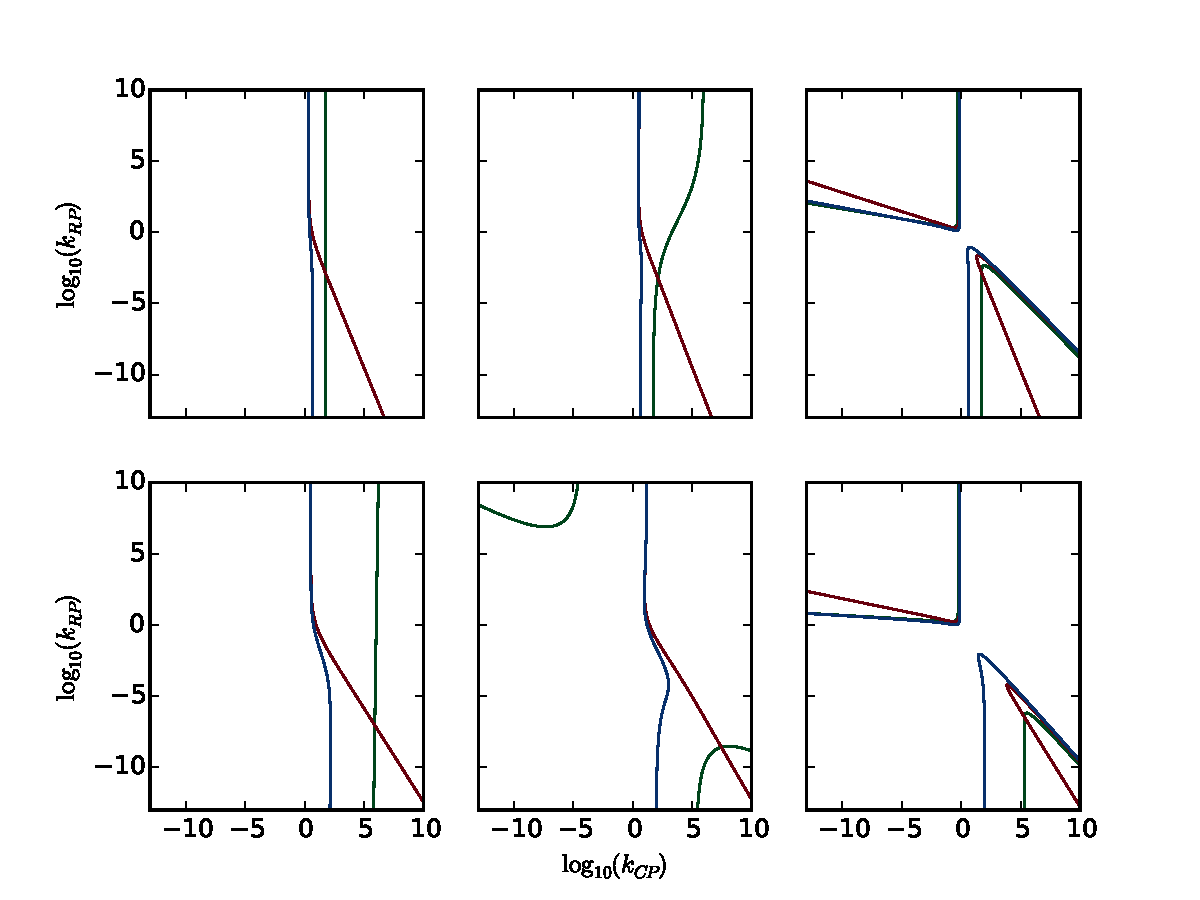
\includegraphics[width = 0.99\textwidth]{./Plots/NecessityCPR.pdf}
  \caption[Condiciones Necesarias $C \to P-R$]{Condiciones necesarias para la invasibilidad del depredador intermedio $C$ sobre el subsistema $P-R$. Las especificaciones se comparten con la figura ~\ref{fig:NC_PCR}}
  \label{fig:NC_CPR}
\end{figure}


Este criterio difiere de los anteriores debido a que los size ratios en este caso no determinan un valor de $m_p$ m\'inimo sino m\'aximo, es decir para size ratios fijos que adem\'as no cumplen con la primera de las condiciones existe un valor de $m_P$ sobre el cual la inserci\'on de $C$ no es posible. La primera condicion en cierta manera independiza el \'exito de la invasi\'on de $C$ de la mortalidad causada por $P$. En la figura ~\ref{fig:Z(IC5)} se grafican distintas curvas de nivel para la Zona $Z(I_{\C \to \PP-\R})$, se observa que la cantidad de combinaciones de size ratios crece con respecto a $m_P$(caso similar con $\kappa_0$), y para $\phi = 2$(lo cual implica funciones unimodales) se incluyen en la zona $k_\CP$ elevados, como se esperaba debido a la disminuci\'on de la eficiencia de captura por parte de $P$. A su vez dependiendo del valor de los size ratios las cotas inferior y superior de la zona pueden estar muy cercanas lo que har\'ia que valores de $m_P$ para los cuales se da la invasi\'on de $P$ a $R$ , a pesar de estar cerca a la cota ser\'ian excluidos de la zona. Esto se da cuando $ q_{0,2} - \xi_3 \approx 0$.


\begin{figure}
  \centering
  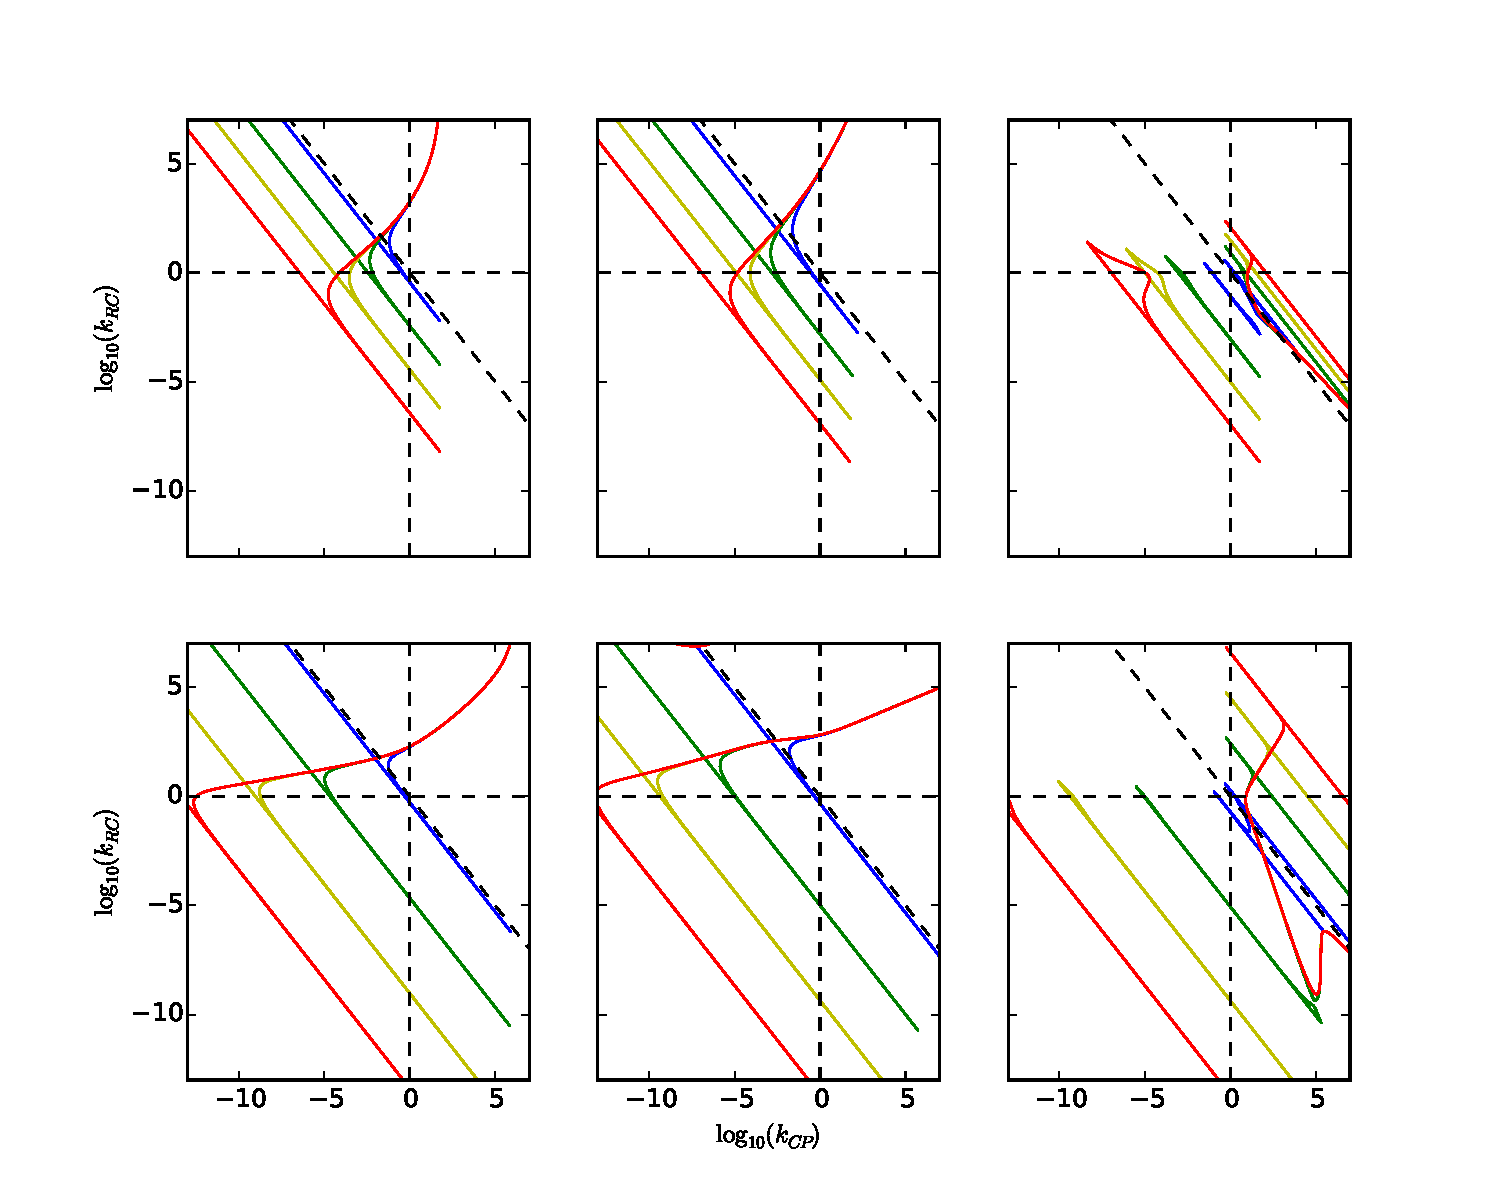
\includegraphics[width = 0.99\textwidth]{./Plots/Z(IC5)AcGrGr.pdf}
  \caption[Env $Z(IC5)$]{\emph{Envolturas de Invasibilidad} para el caso de el depredador intermedio $C$ como invasor frente a una comunidad receptora formada por $R-P$. Las dem\'as especificaciones se comparten con la figura ~\ref{fig:Z(IC2)}.}
  \label{fig:Z(IC5)}
\end{figure}


Juntando ambas zonas anteriores tenemos que la region de \emph{invasibilidad mutua} $Z_{IM} := Z(I_{\C \to \PP-\R}) \cap Z(I_{\PP \to \C-\R})$ , resulta:


\begin{equation}
\mathbf{Z_{IM}} := \{ (k_{\RC},k_{\CP},m_P) \in \mathbb{R}^3_+ / \zeta_4(k_{\RC},k_{\CP}) > m_p > \max \{ \zeta_2(k_{\RC},k_{\CP}) , \zeta_1(k_{\RC},k_{\CP}) , \zeta_3(k_{\RC},k_{\CP}) \}
\end{equation}

La cual hereda todas las caracter\'isticas descritas para los dos casos anteriores, en particular tenemos que size ratios que cumplan la primera condici\'on del caso anterior con $c > 1$ estan exclu\'idas de la zona. A su vez dependiendo del valor de $k_\CP$ y $k_\RC$ las cotas de las zonas pueden estar muy cercanas lo que conllevar\'ia a una gran restricci\'on sobre el valor de $m_P$ posible para que se de esta propiedad. Como era de esperarse para un $m_P$ fijo las combinaciones de size ratios para los cuales esta propiedad se cumple son menores que en casos anteriores(v\'ease figura ~\ref{fig:MutualInv}).


\begin{figure}
  \centering
  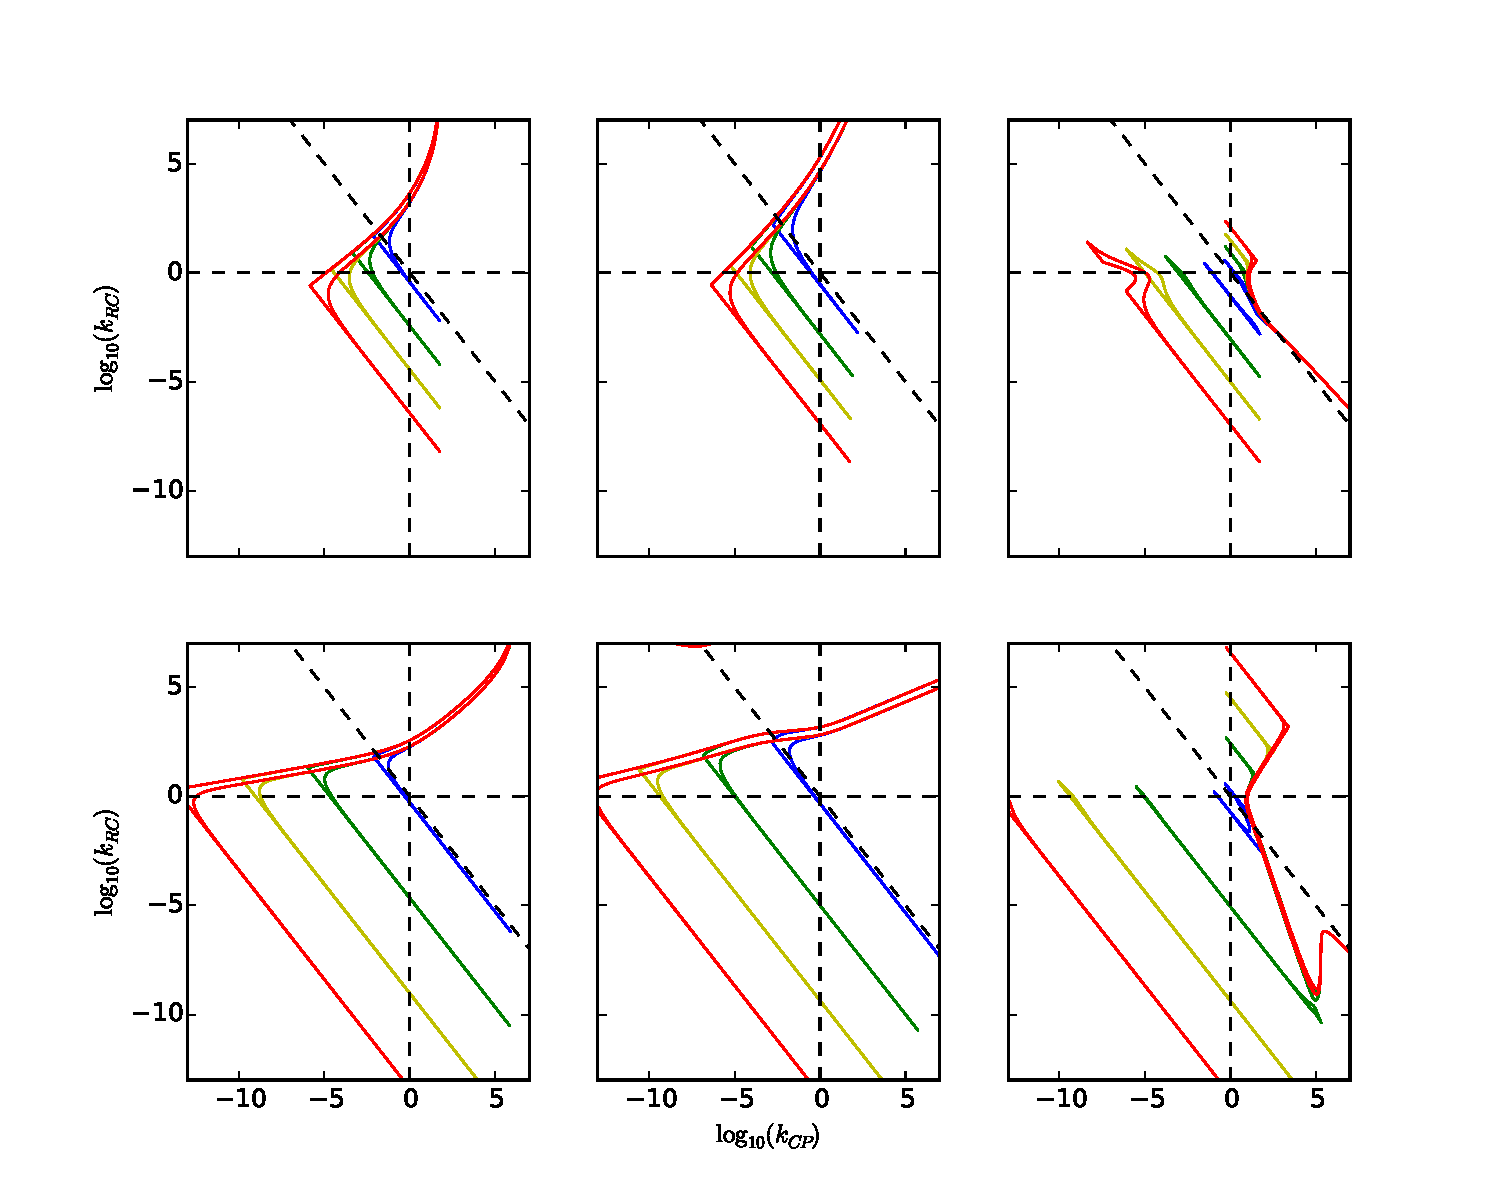
\includegraphics[width = 0.99\textwidth]{./Plots/MutualInvAcGrGr.pdf}
  \caption[Env $I_M$]{\emph{Envolturas de Invasibilidad Mutua} donde ambas sequencias de invasi\'on $S_1$ y $S_2$ dan lugar al m\'odulo completo. Las dem\'as especificaciones se comparten con la figura ~\ref{fig:Z(IC4)}.}
  \label{fig:MutualInv}
\end{figure}


\subsection{Coexistencia}

En el modelo usado una condici\'on necesaria para la existencia de un equilibrio positivo es que el depredador intermedio se mejor competido que el depredador tope, donde la habilidad competitiva se mide con la regla $R$. Esto es:

\begin{equation}
  \frac{q_{0,2}}{\varepsilon_2 \alpha_{0,2} f_2(k_{\RP})} > \frac{q_{0,1} k_{\CP}^{\beta-h}}{\varepsilon_{1} \alpha_{0,1} f_1(k_{\RC})}
\end{equation}

Donde $ h = p_v + 2(D_R -1) p_d$. Recobramos nuevamente la condici\'on $q_{0,2} > \xi_3$, por tanto comparte las propiedades ya descritas previamente. \\
Definimos
\begin{equation}
  \Delta_\epsilon := \varepsilon_2 - \varepsilon_3 \varepsilon_1
\end{equation}
Para $\Delta_\epsilon >0$:
\begin{equation}
  D > 0 \iff m_P^{h + 1 - 2\beta} < \frac{\mu_0}{\mu_1}
\end{equation}

Donde:
\begin{equation}
  \begin{aligned}
    \mu_0 &= \alpha_{0,3}r_0 \varepsilon_3 f_3(k_\CP) \\
    \mu_1 &= k_0 \alpha_{0,1}\alpha_{0,2} \Delta_\varepsilon k_\RP^{1-\beta} k_\CP^{h-1} f_1(k_\RC)f_2(k_\RP)
  \end{aligned}
\end{equation}

En el modelo usado para $D>0$ el equilibrio es positivo si y solo si $\frac{dP}{dt} >0 $ y $\frac{dC}{dt} >0$ , por tanto en este caso tenemos que la zona de coexistencia hereda varias de las propiedades descritas en los dos casos anteriores, m\'as a\'un para $D <0$ tenemos que el equilibrio no puede formarse por una secuencia de invasiones cuyo tiempo entre eventos de colonizaci\'on es tal que la comunidad receptora  llega al equilibrio(como hemos asumido nosotros).



\begin{figure}
  \centering
  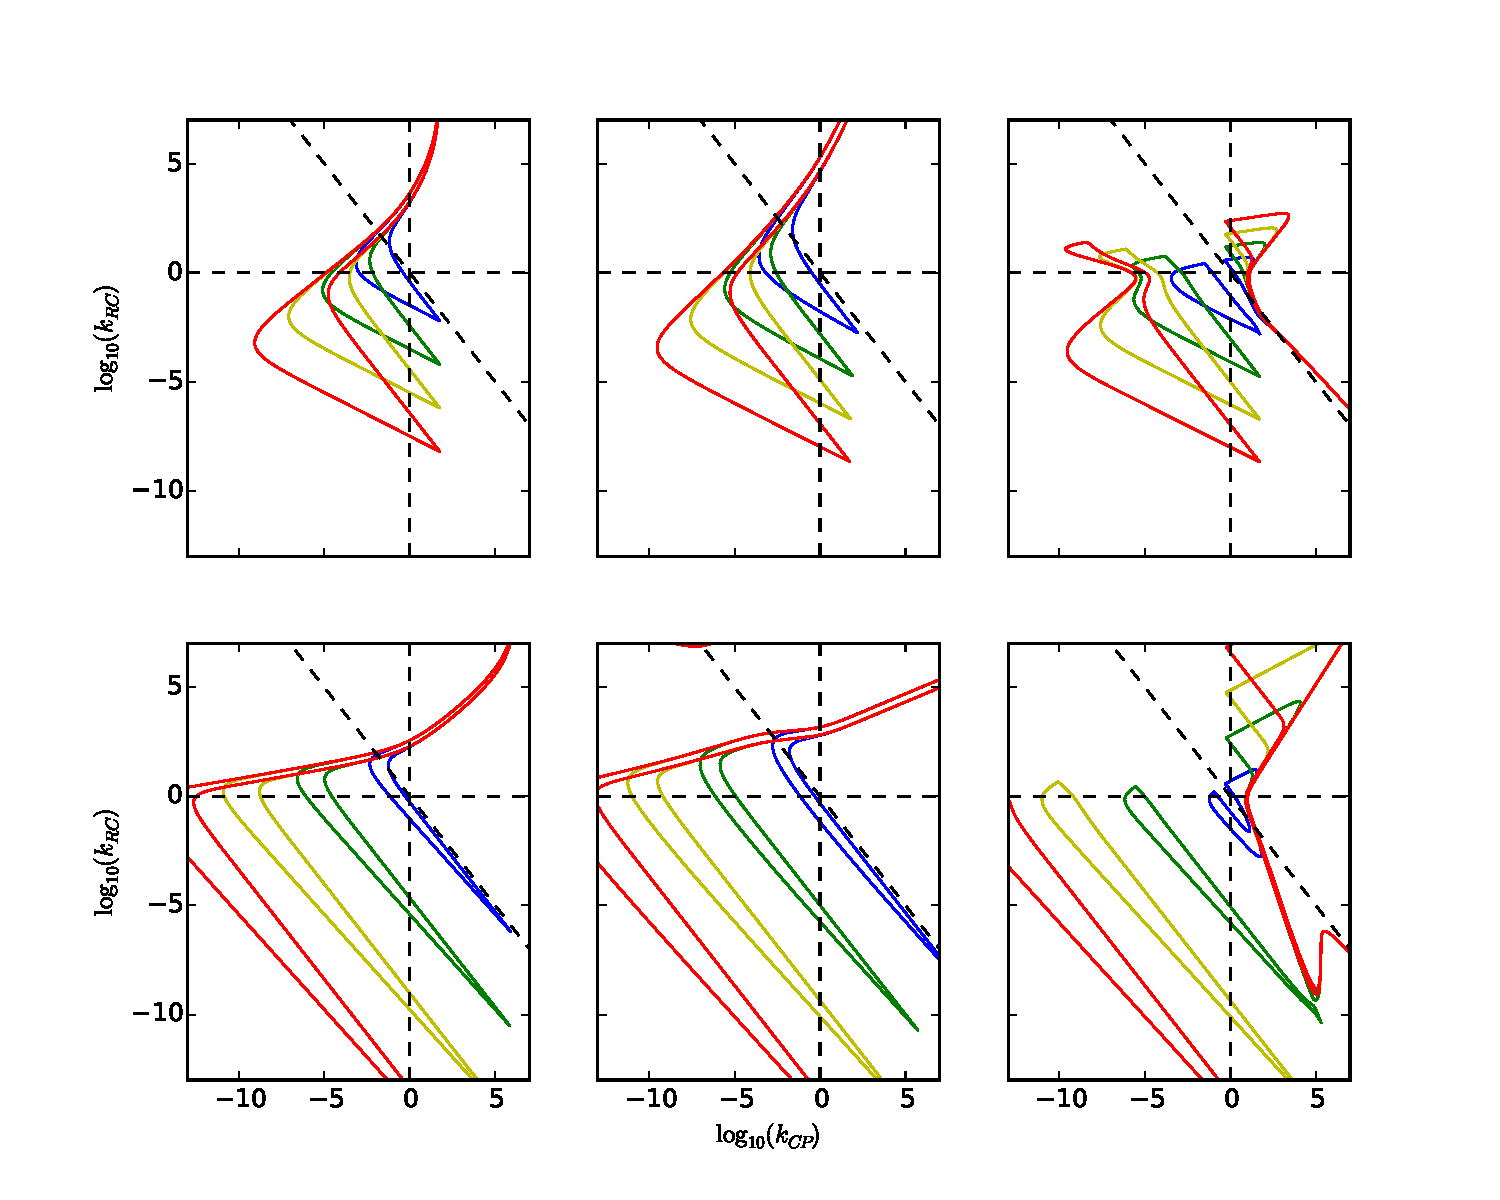
\includegraphics[width = 0.99\textwidth]{./Plots/CoexistenceAcGrGr.pdf}
  \caption[Env $Coexistencia$]{\emph{Coexistencia} donde existe un equilibrio $(R,C,P)$ positivo y este puede ser formado \emph{potencialmente} mediante una secuencia de ensamblaje($S_1$ o $S_2$. Las dem\'as especificaciones se comparten con la figura ~\ref{fig:Z(IC4)}.}
  \label{fig:PSCoexistence}
\end{figure}


\begin{figure}
  \centering
  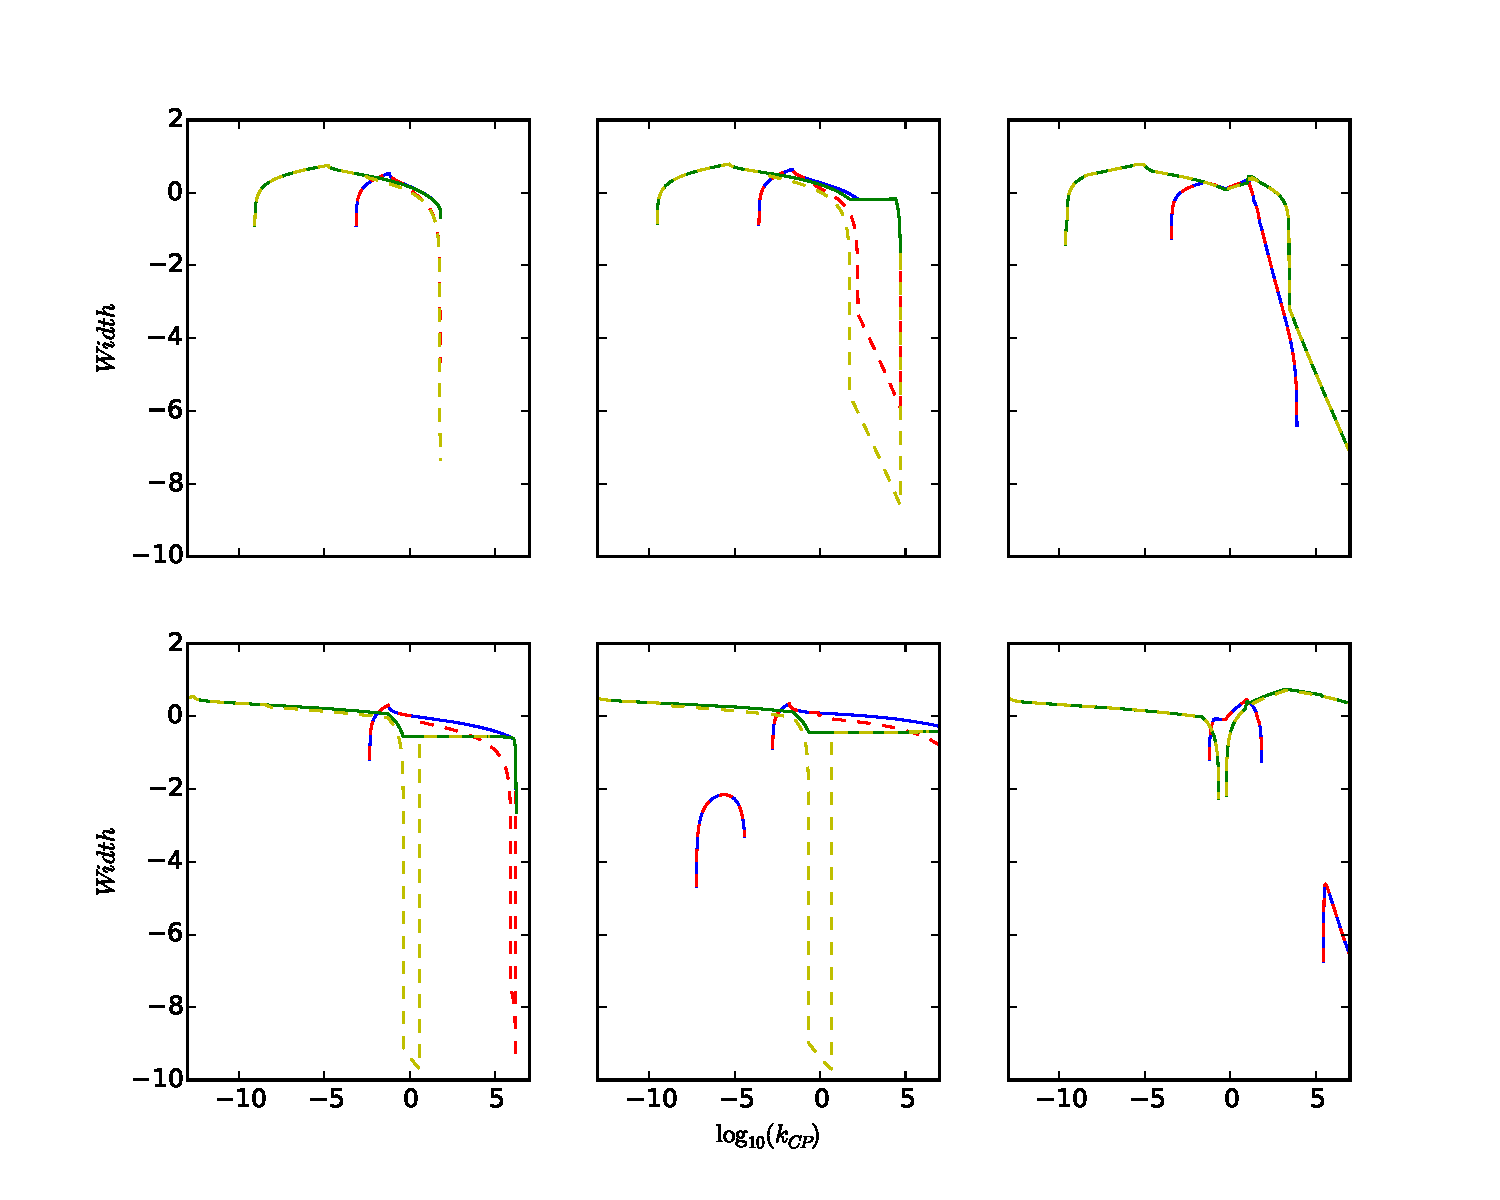
\includegraphics[width = 0.99\textwidth]{./Plots/WidthCoexistenceAcGrGr.pdf}
  \caption[Ancho $Coexistencia$]{Anchos de la zona de \emph{coexistencia} y la zona de \emph{coexistencia estable} respecto a cambios en los valores de $k_{\RC}$.({\hwplotT}) denota \emph{coexistencia} y ({\hwplotK}) \emph{coexistencia estable} . ({\hwplotG}) y  ({\hwplotY}) $10^5 kg$ , ({\hwplotR}) y ({\hwplotB}) para $10^{-10}kg$. Las dem\'as especificaciones se comparten con la figura ~\ref{fig:Z(IC4)}.}
  \label{fig:CoexistenceWidth}
\end{figure}























